\documentclass{article}

\usepackage{graphicx}
\usepackage{varwidth}
\usepackage{xcolor}
\usepackage{colortbl}
\usepackage[mode=buildnew]{standalone}
\graphicspath{{figures/}}
\usepackage[lecture]{random}

\pagestyle{fancy}
\fancyhf{}
\rhead{\textsc{Evelyn Koo}}
\chead{\textsc{Notes (Sp22)}}
\lhead{Data 100}
\cfoot{\thepage}

\begin{document}
\title{Data 100 Notes}
\author{Evelyn Koo}
\date{Summer 2022}
\maketitle
\tableofcontents
\section*{Introduction}
\addcontentsline{toc}{section}{Introduction}
Notes for Data 100, taken using Vim and \LaTeX.
\subsection*{Remarks}
Notes are taken from the slides of the Spring 2022 edition of Data 100.

Some of the figures may be messy or poorly drawn as this is my first time seriously learning TikZ.

\lecture[2022-05-17]{Course Overview}
\subsection{Overview}
\subsubsection{What is Data Science?}
``Data Science'' part of the course name. Fundamentally an interdisciplinary field - it is the application of data-centric, computational, and inferential thinking to understand the world (science) and solve problems (engineering).

Good data analysis is not just simply applying a statistics recipe or using a software. While there are many tools for data science, they are just tools - they do not do the important thinking.

\textbf{Example Questions in Data Science}

\begin{itemize}
\item What show should we recommend to our user to watch?
\item In which markets should we focus our advertising campaign?
\item Is the use of the COMPAS algorithm for prison sentencing fair?
\end{itemize}

\subsubsection{What will you learn in this class?}
``Principles and Techniques'' part of the course name. Course goals:
\begin{itemize}
\item \textbf{Prepare} students for advanced Berkeley courses in data management, ML, and statistics by providing the necessary foundation and context.
\item \textbf{Enable} students to start careers as data scientists by providing experience working with real-world data, tools, and techniques.
\item \textbf{Empower} students to apply computation and inferential thinking to address real-world problems.
\end{itemize}

\textbf{Topics Covered}

\begin{itemize}
\item \textbf{Data Analysis and Visualization}: Using NumPy, Pandas, visualization with matplotlib, Seaborn, plotly; Relational Databases and SQL, Regex
\item \textbf{Statistics}: Sampling, probability, and random variables.
\item \textbf{Machine Learning/Statistics Techniques}: Model designing/loss formulation, linear regression, feature engineering, regularization, bias-variance tradeoff, cross-validation; gradient descent, logistic regression; decision trees and random forests, PCA.
\end{itemize}

\subsection{Data Science Lifecycle}
High-level description of the data science workflow.
\begin{figure}[ht]
\begin{center}
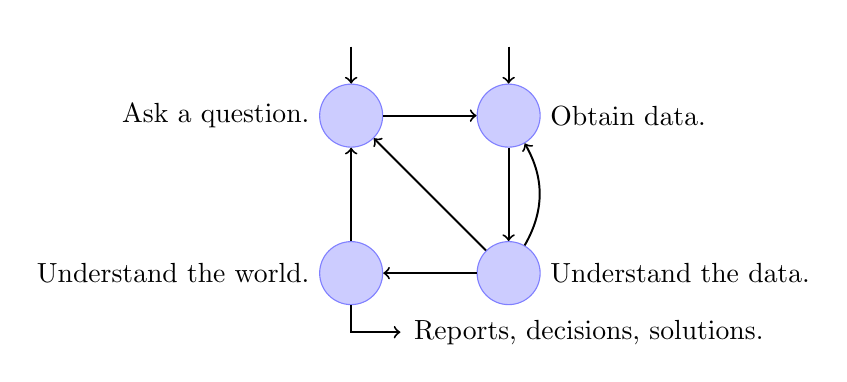
\begin{tikzpicture}
\node (aup) at (-1, 2) [draw=none] {};
\node (dup) at (1, 2) [draw=none] {}; 
\node (result) at (-0.25, -1.75) [draw=none, minimum size=0mm, label={[xshift=-2mm]right:Reports, decisions, solutions.}] {};
\node (ask) at (-1, 1) [circle, draw=blue!50, fill=blue!20, minimum size=8mm, label=left:Ask a question.] {};
\node (data) at (1, 1) [circle, draw=blue!50, fill=blue!20, minimum size=8mm, label=right:Obtain data.] {};
\node (uworld) at (-1, -1) [circle, draw=blue!50, fill=blue!20, minimum size=8mm, label=left:Understand the world.] {};
\node (udata) at (1, -1) [circle, draw=blue!50, fill=blue!20, minimum size=8mm, label=right:Understand the data.] {};
\draw [->, line width=0.25mm] (aup) edge (ask) (dup) edge (data) (ask) edge (data) (data) edge (udata) (udata) edge (uworld) (uworld) edge (ask) (udata) edge (ask);
\draw [->, bend right, line width=0.25mm] (udata) edge (data);
\draw [->, to path = (\tikztostart) |- (\tikztotarget), line width=0.25mm] (uworld) edge (result);
\end{tikzpicture}
\end{center}
\label{fig:ds-lifecycle}
\caption{Diagram of the data science lifecycle. Note the two different entry points.}
\end{figure}
\begin{enumerate}
\item \textbf{Question/Problem Formation} (Ask a question):
\begin{itemize}
\item What do we want to know?
\item What problems are we trying to solve?
\item What are the hypotheses we want to test?
\item What are our metrics for success?
\end{itemize}
\item \textbf{Data Acquisition and Cleaning} (Obtaining Data):
\begin{itemize}
\item What data do we have and what data do we need?
\item How will we sample more data?
\item Is our data representative of the population we want to study?
\end{itemize}
\item \textbf{Exploratory Analysis and Visualization} (Understand the Data):
\begin{itemize}
\item How is our data organized and what does it contain?
\item Do we already have relevant data?
\item What are the biases, anomalies, or other issues with the data?
\item How do we transform the data to enable effective analysis?
\end{itemize}
\item \textbf{Prediction and Inference} (Understand the World):
\begin{itemize}
\item What does the data say about the world?
\item Does it answer our questions or accurately solve the problem?
\item How robust are our conclusions and can we trust the predictions?
\end{itemize}
\end{enumerate}
\begin{example}[Demo: Data Science Lifecycle]{Begin with asking a question (step 1): Who are you?

Then gather and clean data (steps 2 and 3). Our population is Data 100 students, and some sub-questions could be \# of students, majors, year, diversity.

Focus on the final sub-question - diversity. Surveys of data scientists suggest that there are far fewer women:
\begin{center}
\includegraphics[width=0.6\textwidth]{diversitynt.png}
\end{center}

We want to see if this holds in the class (steps 4 and 1). We now have a new question: ``What fraction of students are female?'', and the process repeats itself again.

\tcbline

Now, since we want to find female students, a new question arises: ``Can we estimate a person's sex using their name?'' and we obtain more data: SSN baby names (steps 1, 2, and 3).

Using this data, we try to estimate the fraction of female students in the class (step 4). A possible classifier:
\begin{enumerate}
\item SSN: Proportion of female babies per name.
\item Use step 1 to classify each student name as F, M, or unknown.
\item Average step 2 to get the class proportion of females.
\end{enumerate}

However, the current model doesn't account for uncertainty. Create a new classifier:
\begin{enumerate}
\item SSN: Proportion of female babies per name.
\item For each student name from above:
\begin{enumerate}
\item Pick a number in $[0, 1)$.
\item If 2a is less than the SSN proportion (or 0.5 for Unknown), classify student as F; else M.
\end{enumerate}
\item Average step 2 to get a class proportion of females.
\end{enumerate}
\tcbline
\textbf{Recap}
\begin{itemize}
\item Find Data 100 data.
\item Explore interesting things about the class: names, majors, etc.
\begin{itemize}
\item Get stuck on a question: gender diversity.
\end{itemize}
\item Find more data: US SSN baby names.
\begin{itemize}
\item \textit{Approximate} gender with sex.
\end{itemize}
\item Create a classifier:
\begin{itemize}
\item Simple classifier: classifies names as exactly F/M.
\item Random classifier: all names have some probability of F.
\end{itemize}
\end{itemize}

\textbf{Limitations}
\begin{itemize}
\item US name data - while there are students from around the world here at Berkeley.
\item Names from since 1937; however, most students are born around 2000.
\item No ``rare'' names.
\item Sex as a proxy for gender - gender has been proxied to a binary classification.
\end{itemize}
Class data was \textit{fundamentally insufficent} to answer original question. Currently don't have the data to answer the question. Can survey the students to get the true proportion or use the data we have to get an estimate.
}
\end{example}

\lecture[2022-05-17]{Data Sampling and Probability}
Previously, we mentioned the \href{fig:ds-lifecycle}{data science lifecycle}. Today, we focus on step 2: collecting data. How do we collect data?
\begin{center}
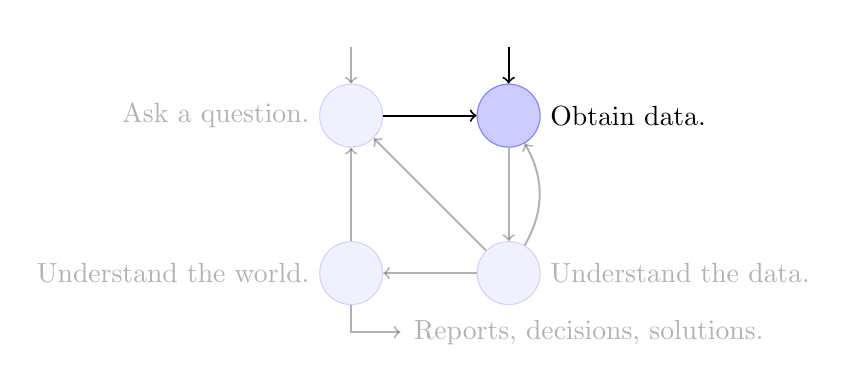
\begin{tikzpicture}
\node (aup) at (-1, 2) [draw=none] {};
\node (dup) at (1, 2) [draw=none] {}; 
\node (result) at (-0.25, -1.75) [draw=none, minimum size=0mm, label={[xshift=-2mm, opacity=0.3]right:Reports, decisions, solutions.}, opacity=0.3] {};
\node (ask) at (-1, 1) [circle, draw=blue!50, fill=blue!20, minimum size=8mm, label={[opacity=0.3]left:Ask a question.}, opacity=0.3] {};
\node (data) at (1, 1) [circle, draw=blue!50, fill=blue!20, minimum size=8mm, label=right:Obtain data.] {};
\node (uworld) at (-1, -1) [circle, draw=blue!50, fill=blue!20, minimum size=8mm, label={[opacity=0.3]left:Understand the world.}, opacity=0.3] {};
\node (udata) at (1, -1) [circle, draw=blue!50, fill=blue!20, minimum size=8mm, label={[opacity=0.3]right:Understand the data.}, opacity=0.3] {};
\draw [->, line width=0.25mm, opacity=0.3] (aup) edge (ask) (data) edge (udata) (udata) edge (uworld) (uworld) edge (ask) (udata) edge (ask);
\draw [->, line width=0.25mm] (dup) edge (data) (ask) edge (data);
\draw [->, bend right, line width=0.25mm, opacity=0.3] (udata) edge (data);
\draw [->, to path = (\tikztostart) |- (\tikztotarget), line width=0.25mm, opacity=0.3] (uworld) edge (result);
\end{tikzpicture}
\end{center}

\subsection{Sampling}

\subsubsection{Censuses and Surveys}
US decennial census - last held in April 2020. Counts \textit{every person} living in all 50 states, DC, and US territories - not just citizens. Mandated by the constitution and participation is required by law.

Important uses of the census:
\begin{itemize}
\item Allocation of federal funds.
\item Congressional representation (update based on population).
\item Drawing congressional/state representative districts.
\end{itemize}

\begin{definition}[Census]{In general, a census is an official count or survey of a population, typically recording various details of individuals.
}
\end{definition}

\begin{definition}[Survey]{A survey is a set of questions; e.g. workers survey individuals and households.

What and how the questions are asked can affect how the respondent answers or whether they answer at all.
}
\end{definition}

\subsubsection{Sampling: Definitions}
While a census is great, it is expensive and difficult to execute (e.g. would all voters be willing to participate in a voting census before an election?). For this, we can use samples.

\begin{definition}[Sample]{A sample is a subset of the population.
\begin{itemize}
\item Often used to make inferences about the population.
\item How the sample is drawn will affect its accuracy.
\item Common sources of error:
\begin{itemize}
\item \textbf{Chance error}: random samples vary from what is expected in any direction.
\item \textbf{Bias}: systematic error in one direction.
\end{itemize}
\end{itemize}
}
\end{definition}
\textbf{Population, Sample, and Sampling Frame}
\begin{itemize}
\item \textbf{Population}: group you want to learn something about.
\item \textbf{Sampling Frame}: list from which the sample is drawn (e.g. if you are sampling people, the sampling frame is the set of all people who can end up in the sample).
\item \textbf{Sample}: who you actually end up sampling; a subset of the sampling frame.
\end{itemize}
\begin{figure}[ht]
\begin{center}
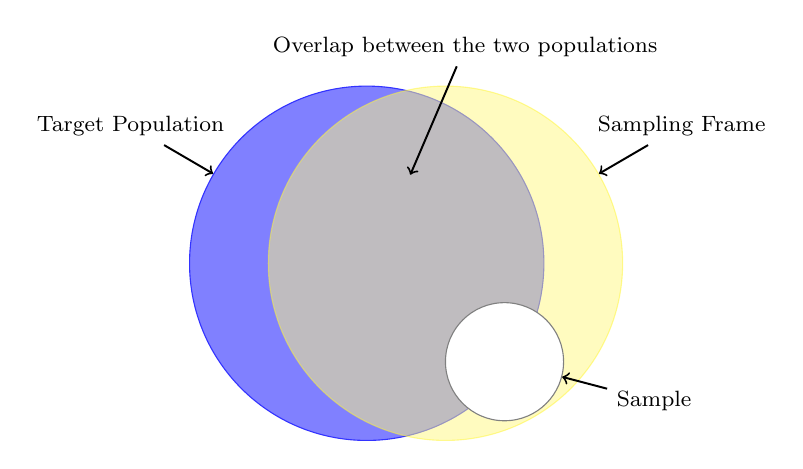
\begin{tikzpicture}
\node[circle, draw=blue!80, fill=blue!50, minimum size=45mm] (target) at (-0.5,0) {};
\node[circle, draw=yellow!80, fill=yellow!50, minimum size=45mm, opacity=0.5] (sframe) at (0.5, 0) {};
\node[circle, draw=black!50, fill=white, minimum size=15mm] (sample) at (1.25, -1.25) {};
\node[draw=none] (ol) at (0.75, 2.75) {\footnotesize Overlap between the two populations};
\node[draw=none] (tp) at (-3.5, 1.75) {\footnotesize Target Population};
\node[draw=none] (sf2) at (3.5, 1.75) {\footnotesize Sampling Frame};
\node[draw=none] (s2) at (3.15, -1.75) {\footnotesize Sample};
\node[draw=none] (dummy) at (0, 1) {};
\draw[->, line width=0.25mm] (sf2) edge (sframe) (s2) edge (sample) (tp) edge (target) (ol) edge (dummy);
\end{tikzpicture}
\end{center}
\caption{Target Population, Sampling Frame, and Sample. Note that there may be people in the sampling frame (and therefore, the sample) which are not part of the population.}
\end{figure}

\subsubsection{Bias: A Case Study}
\textbf{1936 Presidential Election}

Here, President FDR went up for re-election against Alf Landon. Polls were conducted in the months leading up to the election trying to predict the outcome.

One of the polls was from The Literary Digest, a magazine which had successfully predicted the outcome of 5 general elections up till 1936. Their survey was sent to 10 million people from phone books, magazines subscribers, and country club members. This poll got that 43\% of people would choose FDR in the election, but in the actual election, 61\% of people chose FDR.

\textbf{Literary Digest poll: What went wrong?}
\begin{enumerate}
\item Sampling frame was not representative of the US population.
\begin{itemize}
\item Chose people who had phone numbers and subscribed to their magazines or country clubs. 
\item Such people tend to be more affluent and more likely to vote Republican.
\end{itemize}
\item Non-response: only 2.4 million people (24\%) filled out the survey. Who knows how the other 76\% would have responded?
\end{enumerate}

\textbf{Gallup's Poll}

In addition to the Literary Digest poll, George Gallup also made predictions about the 1936 elections. Looking at the table, his result (56\%) was much closer to the actual election and with a smaller sample size.
\begin{center}
\begin{tabular}{@{}lll@{}}
\toprule
     & \% Roosevelt & \# surveyed \\
\midrule
    Election & 61\% & All voters ($\sim$45 million) \\
    Literary Digest Poll & 43\% & 10 million \\
    Gallup's Poll & 56\% & 50 000 \\
    Gallup's prediction of Digest's Poll & 44\% & 3 000 \\
\bottomrule
\end{tabular}
\end{center}
Gallup was even able to predict the Literary Digest's prediction within 1\% using a much smaller sample size. Why?
\begin{itemize}
\item He predicted their sampling frame (phonebook, magazine subscribers, country clubs).
\item So he sampled the same individuals.
\end{itemize}

\textbf{Common Biases}

Samples, while convenient, are subject to chance error and bias.
\begin{itemize}
\item \textbf{Selection Bias}: Systematically avoiding/favoring particular groups. Avoid by examining the sampling frame and the method of sampling.
\item \textbf{Response Bias}: People don't always respond truthfully. Avoid by examining the nature of questions and the method of surveying.
\item \textbf{Non-response Bias}: People don't always respond. Avoid by making surveys short and being persistent - people who don't respond aren't like the people who do.
\end{itemize}
It's likely that the Literary Digest sample was a case of selection bias - they favored choosing those who they could easily access through the phonebook/subscriptions.

\subsection{Probability}
\subsubsection{Probability Samples}
When sampling, go for quality over quantity - don't just go for a big sample (as that can lead to having a big sample that is of poor quality).

\textbf{Common Non-Random Samples}
\begin{itemize}
\item \textbf{Convenience Sample}: choose whoever you can get ahold of (e.g. when trying to measure the weight of mice, choosing whichever mice you can get ahold of as samples to measure weight).
\begin{itemize}
\item Not a good idea for inference.
\item Haphazard $\neq$ random.
\item Sources of bias can be present in ways that you may not think of (e.g. all the convenient samples can be of one group).
\end{itemize}
\item \textbf{Quota Sample}: Specify desired breakdown of various subgroups in population, then choose to reach targets however you can (e.g. Sampling individuals in your town and having the sample match the age distribution from the census).
\begin{itemize}
\item Reaching quotas ``however you can'' is not random.
\item Sample will represent some of the population (e.g. age), but not all of the population (e.g. gender, ethnicity, income may not be well represented in the sample).
\end{itemize}
\end{itemize}
So why sample at random? One thing is to reduce bias (despite this, random samples can still produce biased estimates); however, the main reason is that we can estimate bias and chance error with random samples, allowing us to quantify uncertainty.
\begin{definition}[Probability Sample]{Sample from a random sampling scheme. Has the following properties:
\begin{itemize}
\item Must be able to provide the chance that any specified set of individuals will be in the sample.
\item All individuals in the population need not have the same chance of being selected.
\item Will be able to measure the errors since you know all the probabilities.
\end{itemize}
}
\end{definition}
\begin{example}[]{Suppose there are 3 students: A, B, and D. Sample 2 students with the following procedure:
\begin{itemize}
\item Choose A with probability 1.
\item Choose from $\{B,D\}$ with probability 0.5 each.
\end{itemize}
\textbf{Possible Outcomes:}
\begin{center}
\begin{tabular}{@{}cc@{}}
\toprule
    Subsets of 2 & Probabilities \\
\midrule
    $\{A,B\}$ & 0.5 \\
    $\{A,D\}$ & 0.5 \\
    $\{B,D\}$ & 0 \\
\bottomrule
\end{tabular}
\end{center}
This is a probability sample, though not a great one:
\begin{itemize}
\item Of the 3 people in each population, know the probability (chance) of getting each subset.
\item If we're measuring the average distance students live from campus, then problems arise:
\begin{itemize}
\item The sampling frame does not account for the entire population - only three students.
\item Some \textit{chance error} depending on if the sample is AB or AD.
\item Since we choose A w.p. 1, the sample \textit{biases} towards A's response
\end{itemize}
\end{itemize}
}
\end{example}
\textbf{Common Random Sample Schemes}
\begin{itemize}
\item \textbf{Random Sample with replacement}: sample drawn uniformly at random with replacement.
\item \textbf{Simple random sample (SRS)}: sample drawn uniformly at random without replacement.
\begin{itemize}
\item Each individual/subset of individuals has the same chance of being selected.
\item Each pair has the same chance as every other pair; each triple has the same chance as every other triple (independent).
\end{itemize}
\end{itemize}
\begin{notebox}[]
Random doesn't always mean ``uniformly at random'', but with these examples, it does.
\end{notebox}
\begin{example}[]{Consider the following sampling scheme:
\begin{itemize}
\item Class roster has 1100 students listed alphabetically.
\item Pick one of first 10 students on the list at random.
\item Given the number from previously, sample the student and every 10th student listed after that (e.g. students 8, 18, 28, ...).
\end{itemize}
Determine the following:
\begin{enumerate}
\item Is this a probability sample?
\item Does each student have the same probability of being selected?
\item Is this a simple random sample?
\end{enumerate}
\tcbline
\begin{enumerate}
\item Yes, we can provide the probability of each subset being elected, e.g. $\Pr(S=\{8, 17, \ldots\}) = 0$, $\Pr(S=\{8, 18, \ldots\}) = \frac{1}{10}$.
\item Yes, each student has a 1/10 chance of being selected.
\item No, the samples are not independent - the probabilities are different for each pair. As noted above, $\Pr(\{8, 17\} \in S) = 0 \neq \Pr(\{8, 18\} \in S) = \frac{1}{10}$.
\end{enumerate}
}
\end{example}
Often, in data science, the population is large, but we can only afford to sample a small number of individuals. If the population is relatvely large compard to the sample, then sampling with and without replacement are pretty much the same.
\begin{example}[Sampling with/without Replacement]{Suppose there are 10 000 people in the population; 7 500 who like Snack 1 and 2 500 who like Snack 2. Find the probability of all people in a sample of 20 liking Snack 1 with and without replacement.
\tcbline 
\begin{itemize}
\item \textbf{SRS/Without Replacement}: first probability is $\frac{\text{\# people who like S1}}{\text{Population}}$, then $\frac{\text{\# people who like S1}-i+1}{\text{Population}-i+1}$ for the $i$th person.
\[
P(\text{All 20 people like S1}) = \left(\frac{7500}{1000}\right) \left(\frac{7499}{9999}\right) \cdots \left(\frac{7482}{9982}\right) \left(\frac{7481}{9981}\right) \approx 0.03153   
.\] 
\item \textbf{With Replacement}: all probabilities are $\frac{\text{\# people who like S1}}{\text{Population}} = \frac{3}{4}$.
\[
P(\text{All 20 people like S1}) = \left(\frac{3}{4}\right)^{20} \approx 0.003171
.\] 
\end{itemize}
The results are close as the without replacement proportion remains close to the with replacement proportion; however, it is easier to calculate the probability without replacement.
}
\end{example}
\textbf{Recap}

If a sample was randomly sampled with replacement from a population:
\begin{itemize}
\item It is a probability sample.
\item We can quantify error and bias.
\item Given the population distribution, we can compute the probability of getting a particular sample.
\end{itemize}
\begin{notebox}[]
We almost never know the population distribution unless we take a census. However, framing allows us to quantify our uncertainty in any analysis/inference using our sample.
\end{notebox}

\begin{example}[Application: The Gallup Poll Today]{tbc
}
\end{example}

\subsubsection{Multinomial and Binomial Probabilities}
Binomial and multinomial probabilities arise when we: 
\begin{itemize}
\item Sample at random with replacement. (Think of as same trial)
\item Sample a fixed number (n) times.
\item Sample from a categorical distribution: 2 - binomial, $>2$ - multinomial.
\begin{center}
\begin{tabular}{@{}lll@{}}
\toprule
    & Binomial & Multinomial \\
\midrule
    \# Categories & 2 categories & $>2$ categories \\
    Example & Bag of Marbles: 60\% blue, 40\% not blue & Bag of Marbles: 60\% blue, 30\% green, 10\% red \\
\bottomrule
\end{tabular}
\end{center}
\end{itemize}
\textbf{Goal}: count the number in each category that end up in our sample. \mintinline{text}{np.random.multinomial} returns these counts.

\begin{example}[Binomial Probability]{Suppose we sample at random with replacement 7 times from a bag of marbles (60\% blue - b, 40\% not blue - n). Define the following events:
\begin{itemize}
\item A: Get the following marbles in the following order: bnbbbnn.
\item B: Get 4 blue marbles and 3 not blue marbles.
\end{itemize}
Find $\Pr(A)$. Is $\Pr(B)$ greater than, the same as, or smaller than $\Pr(A)$?
\tcbline 
\begin{align*}
    \Pr(A) &= (0.6) \cdot (0.4) \cdot (0.6)^3 \cdot (0.4)^2 \\
    &= (0.6)^4(0.4)^3
.\end{align*}
$\Pr(B) > \Pr(A)$. This is since A is a specific case of B (4 blues, 3 not blues). B could have any permutation of the marbles as long as there are 4 blue marbles out of 7. Therefore, there are more outcomes under event B, and since each outcome is uniform, the probability of B (multiple outcomes) happening is greater than A (one outcome).
\[
\Pr(B) = \left( \frac{7!}{4!3!} \right) (0.6)^4 (0.4)^3 = \binom{7}{4} (0.6)^4 (0.4)^3
.\]
}
\end{example}

\begin{example}[Multinomial Probability]{Sample with replacement 7 times from a bag of marbles (60\% blue, 30\% green, 10\% red). Define the following events:
\begin{itemize}
\item A: Get the following marbles in the following order: bgbbbgr.
\item B: Get 4 blue marbles, 2 green marbles, and 1 red marble.
\end{itemize}
\tcbline 
To find A, use the product rule for independent marble draws:
\begin{align*}
    \Pr(A) &= (0.6) \cdot (0.3) \cdot (0.6)^3 \cdot (0.3) \cdot (0.1) \\
    &= (0.6)^4 (0.3)^2 (0.1) \\
.\end{align*}
For B, the result is A (specific, ordered combination) by the number of outcomes with the exact marble distribution:
\[
\Pr(B) = \left( \frac{7!}{4!2!1!} \right) (0.6)^4 (0.3)^2 (0.1) \\
.\]
}
\end{example}
\textbf{Generalization of Multinomial Probability}: For drawing with replacement n times from a population broken into m categories where $\sum_{i \in m} p_m = 1$ (i.e. each category has proportion $p_i$ of the population). Then, the multinomial probability of drawing $k_i$ individuals from each category $i$ is:
\[
    \frac{n!}{k_1!k_2!\ldots k_m!} p_1^{k_1} p_2^{k_2} \ldots p_m^{k^m}
.\]
\begin{notebox}[Derivation of Multinomial Probability Coefficient]
Looking back at the previous example, how did we get $\frac{7!}{4!2!1!}$? Here are a few ways to think of it:
\begin{enumerate}
    \item Start with 7 open positions, then choose 4, which is then $\binom{7}{4}$. Now 3 positions remain for green marbles, of which you choose 2, which is then $\binom{3}{2}$. Now, one position remains for red marbles, which you choose 1, which is then $\binom{1}{1}$.
\[
\binom{7}{4} \cdot \binom{3}{2} \cdot \binom{1}{1} = \frac{7!}{4!3!} \cdot \frac{3!}{2!1!} \cdot \frac{1!}{1!0!} = \frac{7!}{4!3!1!}
.\]
\item Start with 7 open positions, want to arrange marbles in as many ways as possible, which is 7! to begin with. However, since there are 4 blue marbles (identical, meaning putting blues in any 4 places would be just one arrangement), you can divide by 4!, and you can do the same for 2 greens (divide by 2!).
\end{enumerate}
\end{notebox}

\lecture[2022-05-20]{Pandas I}
\definecolor{gold}{rgb}{0.76, 0.66, 0.06} 
Tabular data is one of the most common data formats and the primary focus of Data 100. In Data 8, we used the \mintinline{text}{Table} class of the \mintinline{text}{datascience} library. Here in Data 100, we use the \mintinline{text}{DataFrame} class of the \mintinline{text}{Pandas} library.
\begin{figure}[ht]
\begin{minipage}{0.5\textwidth}
\includegraphics[width=\textwidth]{dataframe.png}\centering
\end{minipage}
\begin{minipage}{0.5\textwidth}
\begin{center}
\includestandalone{figures/3-df}
\end{center}
\end{minipage}
\caption{Left: A sample Pandas DataFrame. Right: A generic DataFrame with a statistical interpretation; rows are samples from the population, columns are features that each sample has.}
\end{figure}
\begin{notebox}[Pandas DataFrame API]
Pandas DataFrame API (application programming interface, or set of applications supported by the class) is very large. When dealing with problems, Google them - they are often found in the documentation or stack overflow.

\href{https://pandas.pydata.org/docs/reference/api/pandas.DataFrame.html}{\color{blue}API Reference}
\end{notebox}

\subsection{Indexing}
One of the most basic tasks of manipulating a DataFrame is to extract rows/columns. Since the Pandas API is very large, this means there are many ways to do things.

Additionally, there is a lot of ``syntactic sugar'' - methods that may be useful and lead to concise code that are not necessary for the library to function (e.g. \mintinline{text}{.head}/\mintinline{text}{.tail}, which select the first/last n rows).

\subsubsection{head/tail}
General Form: \mintinline{text}{df.(head|tail)(<num_rows>)}

Selects the first/last n rows. \mintinline{text}{df.head(5)} is equivalent to \mintinline{text}{df.loc[[0:4]]}, while \mintinline{text}{df.tail(5)} is equivalent to \mintinline{text}{df.loc[[-5:]]}. 

\subsubsection{loc}
General Form: \mintinline{text}{df.loc[<rows>, <cols>]}.

Fundamentally, \mintinline{text}{loc} selects items by label - the bolded text in the top (column names/features) and left (row numbers/samples). Can pass in a list, slice, or single value into \mintinline{text}{loc}.

To select all columns, omit the second argument. To select all rows, pass in \mintinline{text}{:} as the first argument - it is equivalent to selecting the entire array of row numbers.

\begin{figure}[ht]
\begin{minipage}{0.5\textwidth}
\includegraphics[width=\textwidth]{ex-loc.png}\centering
\end{minipage}
\begin{minipage}{0.5\textwidth}
\includegraphics[width=\textwidth]{ex-loc2.png}\centering
\end{minipage}
\caption{Left: selecting different values with \mintinline{text}{loc}. Right: selecting all rows with \mintinline{text}{loc}.}
\end{figure}

\subsubsection{iloc}
General Form: \mintinline{text}{df.iloc[<row-nums>, <col-nums>]}.

Fundamentally, \mintinline{text}{iloc} selects items by number. For rows, this is the same as the label; however, this is not always the case for columns. Like \mintinline{text}{loc}, \mintinline{text}{iloc} can have single values, slices (\mintinline{text}{[<start-num, end-num)}), or arrays passed in as arguments.

And just like \mintinline{text}{loc}, to select all rows, pass in \mintinline{text}{:}, and to select all columns, omit the second argument.

\begin{figure}[ht]
\begin{minipage}{0.5\textwidth}
\includegraphics[width=\textwidth]{ex-iloc.png}\centering
\end{minipage}
\begin{minipage}{0.5\textwidth}
\includegraphics[width=\textwidth]{ex-iloc2.png}\centering
\end{minipage}
\caption{Left: selecting different values with \mintinline{text}{iloc}. Note how instead of column names, we used column numbers. Right: selecting all rows with \mintinline{text}{iloc}.}
\end{figure}

\begin{notebox}[loc vs. iloc]
When deciding between \mintinline{text}{loc} and \mintinline{text}{iloc}, usually \mintinline{text}{loc} is the better choice - it's safer (e.g. will select the right columns if columns are mixed up) and more legible (e.g. \mintinline{text}{["colname1", "colname2"]} over \mintinline{text}{[1, 2]}).

However, \mintinline{text}{iloc} can still be useful - e.g. it would make more sense to index into the middle of a dataframe with \mintinline{text}{iloc}.
\end{notebox}

\subsubsection{[]}
General Form: \mintinline{text}{df[(<row-nums>|col-labels|col-label)]}.

Unlike \mintinline{text}{loc} and \mintinline{text}{iloc}, \mintinline{text}{[]} only takes in one argument rather than rows or columns. The use of \mintinline{text}{[]} changes on the context - i.e., it is context sensitive.
\begin{itemize}
\item For a slice of numbers, it returns the numbered rows.
\item For a list of column names or a single column name, it returns the column(s) in question.
\end{itemize}

\begin{figure}[ht]
\begin{minipage}{0.33\textwidth}
\includegraphics[width=\textwidth]{ex-brac.png}\centering
\end{minipage}
\begin{minipage}{0.34\textwidth}
\includegraphics[width=\textwidth]{ex-brac2.png}\centering
\end{minipage}
\begin{minipage}{0.33\textwidth}
\includegraphics[width=\textwidth]{ex-brac3.png}\centering
\end{minipage}
\caption{\mintinline{text}{[]} in different contexts.}
\end{figure}

\begin{example}[]{Suppose we have the following dataframe \mintinline{text}{weird}:
\begin{center}
\begin{tabular}{@{}crr@{}}
     & \textbf{0} & \textbf{1} \\
\midrule
    \textbf{0} & topdog & topcat \\
    \rowcolor[gray]{0.85}\textbf{1} & botdog & botcat \\
\end{tabular}
\end{center}
What does the following return:
\begin{itemize}
\item \mintinline{text}{weird[1]}
\item \mintinline{text}{weird["1"]}
\item \mintinline{text}{weird[1:]}
\end{itemize}
\tcbline
\begin{itemize}
\item \mintinline{text}{weird[1]}: single column number, so it should return column 1 - i.e. the first column "0".
\begin{center}
\begin{tabular}{@{}cr@{}}
      & \textbf{0} \\
\midrule
    \textbf{0} & topdog \\
    \rowcolor[gray]{0.85} \textbf{1} & botdog \\
\end{tabular}
\end{center}

\item \mintinline{text}{weird["1"]}: single column label, so it should return column "1".
\begin{center}
\begin{tabular}{@{}cr@{}}
      & \textbf{1} \\
\midrule
    \textbf{0} & topcat \\
    \rowcolor[gray]{0.85} \textbf{1} & botcat \\
\end{tabular}
\end{center}

\item \mintinline{text}{weird[1:]}: row slices, so just the first row and beyond.
\begin{center}
\begin{tabular}{@{}crr@{}}
     & \textbf{0} & \textbf{1} \\
\midrule
    \textbf{1} & botdog & botcat \\
\end{tabular}
\end{center}

\end{itemize}
}
\end{example}
\begin{notebox}[\normalfont \mintinline{text}{[]} \textbf{Usage and Dot Notation}]
Whereas \mintinline{text}{loc} and \mintinline{text}{iloc} both accept multiple arguments, \mintinline{text}{[]} does not and selects based on context. Therefore, the syntax is more precise and preferred for real world practice compared to \mintinline{text}{loc}.

Another way to index is with dot notation; more info can be found \href{https://www.dataschool.io/pandas-dot-notation-vs-brackets/}{\color{blue}here}.
\end{notebox}

\subsection{DataFrames, Series, and Indices}
Notice in the previous examples above, if we select only a single column, the notebook returns a different format. This is since the return output is a Series and not a DataFrame.

\begin{minted}{python}
type(elections) # DataFrame
type(elections["Candidate"]) # Series
\end{minted}

This leads into the Pandas data structures. Here are the three fundamental data structures in Pandas:
\begin{itemize}
\item \textbf{DataFrame}: 2D Tabular Data.
\item \textbf{Series}: 1D single-column/columnar data.
\item \textbf{Index}: sequence of row labels.
\end{itemize}
We can think of a dataframe as a collection of series that all have the same index.

Indices are not necessarily row numbers; they can also be non-numeric and have names, e.g. State. They also do not have to be unique.

However, column names are almost always unique. (e.g. it would not make sense to have two columns with the same name, but you can force duplicate columns to have them have the same column name).

If you want row/column labels: you can use \mintinline{text}{df.index} for row labels and \mintinline{text}{df.columns} for column labels.
\begin{notebox}[Getting a DataFrame instead of a Series]
If you want a DataFrame instead of a Series input, there are two ways to do so:
\begin{itemize}
\item \mintinline{text}{Series.toFrame()} method.
\item Enclose the single column of interest in a list (e.g. \mintinline{text}{df[[<col-name>]]} as opposed to \mintinline{text}{df[col-name]})
\end{itemize}
\end{notebox}

\subsection{Conditional Selection}
\mintinline{text}{loc} also supports Boolean array input (usually generated by using logical operators on Series). This can be combined with operators, allowing for filtering with multiple criteria
\begin{minted}{python}
elections[elections["Party"] == "Independent"] # checks the Party series for each entry, keeps the entries which the party is independent

elections[(elections["Result"] == "win") & (elections["%"] < 47)] # checks if the election result is a win and if the winning percent is less than 47%
\end{minted}
\begin{example}[]{Which of the following statements returns a DataFrame of the first 3 candidate names only for candidates that won more than 50\% of the vote?
\tcbline
Using \mintinline{text}{loc}: select all the candidates (rows) that have an election percent > 50, choose candidate, year columns, first three rows that satisfy the condition (head).

End Code: \mintinline{text}{elections.loc[[elections['%'] > 50, ["Candidate", "Year"]].head(3)}
}

Using \mintinline{text}{iloc}: The columns in question are candidate (0) and Year (3), and the first three rows that satisfy the conditions are 0, 3, 5. Therefore, the end code should be \mintinline{text}{elections.iloc[[0, 3, 5], [0, 3]]}.
\end{example}

While boolaen array selection is useful, it can lead to overly verbose code when there are complex selections. There are many alternative functions to make the code more concise:
\begin{itemize}
\item \mintinline{text}{.isin}: returns True if the row value is in an array of results.
\item \mintinline{text}{.str.startswith}: return True if the row value starts with the string provided.
\item \mintinline{text}{.query}: Similar to SQL queries select keyword (select rows which fit the criteria). can access Python variables with \mintinline{text}{@<var-name>}.
\item \mintinline{text}{.groupby.filter}: to be discussed in the next lecture.
\end{itemize}

\begin{minted}{python}
# original, verbose code
elections[(elections["Party"] == "Anti-Masonic")  | 
          (elections["Party"] == "American")      |
          (elections["Party"] == "Anti-Monopoly") |
          (elections["Party"] == "American Independent")]

# .isin
a_parties = ["Anti-Masonic", "American", "Anti-Monopoly", "American Independent"]
elections[elections["Party"].isin(a_parties)]
# .str.startswith
elections[elections["Party"].str.startswith("A")]
# query - select rows of elections after 2000 and the result is a win 
elections.query('Year >= 2000 and Result == "win"')
# query with @
parties = ["Republican", "Democratic"]
elections.query('Result == "win" and Party not in @parties') # select winners that don't belong to republican/democratic parties
\end{minted}

\subsection{Utility Functions}
Pandas Series/DataFrames support mathematical, NumPy, and built-in functions as long as the data is numerical. Additionally, Pandas has its own utility functions:
\begin{itemize}
\item \mintinline{text}{size/shape}: size returns the amount of data entries (rows by columns), while shape returns the shape (rows, columns).
\item \mintinline{text}{describe}: gives a brief description of the numerical data, returning the count, mean/stdev, and 5 points (min, 25\%, 50\%, 75\%, and max).
\item \mintinline{text}{sample}: samples a random selection of rows without replacement (add \mintinline{text}{replace=True}) for replacement. Can be chained with other methods and operators (e.g. \mintinline{text}{query}, \mintinline{text}{iloc}, etc.).
\item \mintinline{text}{Series.value_counts}: counts the number of occurences of each unique value (returned as a series of value-count).
\item \mintinline{text}{Series.unique}: returns an array of all unique values in a Series.
\item \mintinline{text}{sort_values}: sorts values in a Series or a DataFrame (must list column on which to sort for a DataFrame) in ascending order (for descending order, set \mintinline{text}{ascending=False}).
\end{itemize}


\lecture[2022-05-21]{Pandas II: Grouping, Aggregation, Pivot Tables Merging}

\subsection{Adding, Modifying, and Removing Columns}
Previously, we saw how we could find the most popular male names in California using \mintinline{text}{query} and sorting the result.

\begin{minted}{python}
babynames.query("Sex ==M and Year == 2020").sort_values("Count", ascending=False) # chooses only rows from 2020 which are male, then sort in descending order
\end{minted}

\begin{figure}[ht]
\includegraphics[width=0.4\textwidth]{4-sort1.png}\centering
\end{figure}

However, how can we find the longest names? If we sort by the names column, it will just return the names in reverse alphabetical order. After some searching, it turns out you can add in a \mintinline{text}{key} parameter which tells Pandas how to sort the values in the column.

\begin{minted}{python}
# start process - sorts names by alphabetical order
babynames.query("Sex == M and Year == 2020").sort_values("Name", ascending=False)
# new code - add key of baby name length
babynames.query("Sex == M and Year == 2020").sort_values("Name", key=lambda name: name.str.len(), ascending=False)
\end{minted}

\begin{figure}[ht]
\begin{minipage}{0.5\textwidth}
\includegraphics[width=0.65\textwidth]{4-sort2.png}\centering
\end{minipage}
\begin{minipage}{0.5\textwidth}
\includegraphics[width=0.65\textwidth]{4-sort3.png}\centering
\end{minipage}
\caption{The first approach only yields the names in reverse alphabetical order, but sorting with the \mintinline{text}{key} parameter yields the desired result.}
\end{figure}

However, this wasn't a feature until 2020. Prior to that, we would need to come up with another solution: 
\begin{itemize}
\item Create a temporary column getting the length of the baby name.
\begin{itemize}
\item Create a new series with only lengths.
\item Add the series to the dataframe.
\end{itemize}
\item Sort using that column.
\item Drop the temporary column. (General Form: \mintinline{text}{df.drop(<name>, (axis="columns"))})
\end{itemize}

\begin{minted}{python}
# creating a new column 
babynames["name_lengths"] = babynames["Name"].str.len() # new series - applies len to the Name series, then assigns the series "name_lengths" to the dataframe as a column
babynames = babynames.sort("name_lengths", ascending=False) # sort by name_length columns in descending order
babynames = babynames.drop("name_lengths", axis="columns") # drop the column - add axis = "columns" to specify it is a column (default drop rows)
\end{minted}

\subsubsection{Sorting by Arbitrary Functions}
To sort by arbitrary functions (e.g. \# occurrences of ``dr'' and ``ea'' in a string), use \mintinline{text}{Series.map} method. (Think of the \mintinline{text}{tbl.apply()} method in datascience)

\begin{minted}{python}
def dr_ea_count(string):
    return string.count("dr") + string.count("ea")

babynames["dr_ea_count"] = babynames["Name"].map(dr_ea_count) # Series.map(<func>)
babynames.sort_values("dr_ea_count", ascending=False)
\end{minted}
\begin{figure}[ht]
\includegraphics[width=0.5\textwidth]{4-map.png}\centering
\end{figure}

\subsection{Group By}
Let's try to find the female baby name whose popularity has fallen the most using RTP (ratio to peak - current number over peak number in a year).

e.g. for the name ``Jennifer'' measured in 2020, there were 172 Jennifers over the peak of 6064 Jennifers in 1972. Therefore, the RTP is $\frac{172}{6064} = 0.0233$.
\begin{figure}[ht]
\includegraphics[width=0.75\textwidth]{4-rtp.png}\centering\caption{Graph of the amount of Jennifers each year.}
\end{figure}

Here's how to do it in Pandas:
\begin{minted}{python}
max_j = max(babynames.query("Name == 'Jennifer' and Sex == 'F'")["Count"]) # max on the count series based on the query (females born named Jennifer)
cur_j = babynames.query("Name == 'Jennifer' and Sex == 'F'")["Count"].iloc[-1] # same query, select count series, choose the last row
rtp = cur_j / max_j # find the rtp - current vs max

# simplifying
def ratio_to_peak(series):
    return series.iloc[-1] / max(series) # current / max 

j_counts = babynames.query("Name == Jennifer and Sex == 'F'")["Count"]
ratio_to_peak(j_counts) # returns the same results as the rtp variable 
\end{minted}

What about finding the RTP for every name and not Jennifer? A possible way is to create a dictionary of RTPs and get the RTP for each unique name.
\begin{minted}{python}
#build dictionary where each entry is the rtp for a given name, e.g. rtps["jennifer"] should be 0.0231
rtps = {}
for name in babynames["Name"].unique(): # use Series.unique to get an array of unique values in a series
    counts_of_current_name = female_babynames[female_babynames["Name"] == name]["Count"] # choose the rows corresponding to the correct name
    rtps[name] = ratio_to_peak(counts_of_current_name)

#convert to series
rtps = pd.Series(rtps)
\end{minted}
However, this approach is very slow and more complicated. The next method takes advantage of \mintinline{text}{.groupby} and \mintinline{text}{.agg}.

\begin{minted}{python}
female_babynames.groupby("Name").agg(ratio_to_peak) # group by column Name, aggregate through the rtp function
# data 8 approach 
female_babynames.group("Name", ratio_to_peak)
\end{minted}

\begin{notebox}[]
The second method (using \mintinline{text}{.groupby} and the Pandas API) is preferred and the one you should be using - you should never be writing code with loops or list comprehensions on Series.
\end{notebox}



\subsection{Pivot Tables}

\subsection{Joining Tables}





\end{document}
